\clearpage
\section{Small-interval fits and the leading-power test}
\label{sec:fits}
\subsection{Data selection and coefficient convention}
\label{sec:fit-selection}
The active mixture data use the grid in Eq.~\eqref{eq:extended-grid},
$\ell=6,\ldots,10$, and $p=1/2$. Let $x=\ell/N$ for the small
interval $A$, and $y=\ell/N$ for the small complement of the large
interval $B$. The common fitting windows are
\begin{align}
 W_x^{\rm Ising}&=(0,0.02],& W_x^{\rm boson}&=(0,0.1],\nonumber\\
 W_y^{\rm Ising}&=(0,0.002],& W_y^{\rm boson}&=(0,0.005].
 \label{eq:common-fit-windows}
\end{align}
Each window is shared by all six ordered pairs and by Free, $F_1$,
and $F_2$ for its CFT and interval type. Zero is an open lower bound;
there is no observation at zero. The two small-interval windows are
frozen. The large-boson upper cutoff is prescribed as $0.005$; the updated
coefficient and neighboring-cutoff checks are documented in
Appendix~\ref{sec:common-window-results}. In this revision,
the large-boson cutoff changes from $0.0047$ to $0.005$; the other
three windows are unchanged.
Every full fit and every omitted-size training set has at least forty
distinct $(N,\ell)$ observations. Exact counts and sampled endpoints
are in Appendix~\ref{sec:window-comparison}.
The overview figures show data through $x,y=0.20$ so the entire fitted
range is visible, with excluded data shaded. Per-pair figures in
Sec.~\ref{sec:window-selection} also provide fitting-window zooms.
Historical primary-to-primary comparisons on $N\leq256$ retain their
separately stated fitting window.
\begin{longtable}{llrrrrr}
\caption{Active mixture geometries, with all $\ell=6,\ldots,10$ at each listed size. The full grids are Eq.~\eqref{eq:extended-grid}. Counts are per direction. The four common fitting windows are Eq.~\eqref{eq:common-fit-windows}; all figures show fractions through $0.2$. Historical $\ell=11,12$ values remain archived and are excluded from this revision.}
\label{tab:scaling-grid}\\\toprule
Interval & CFT & $N_{\max}$ & Retained & Fit & Shown & Minimum fraction\\\midrule
\endfirsthead
\toprule
Interval & CFT & $N_{\max}$ & Retained & Fit & Shown & Minimum fraction\\\midrule
\endhead
\bottomrule\endfoot
small & ising & 8192 & 1650 & 1255 & 1645 & $7.324\!\times\!10^{-4}$\\
small & boson & 16384 & 630 & 598 & 625 & $3.662\!\times\!10^{-4}$\\
large & ising & 8192 & 1650 & 260 & 1645 & $7.324\!\times\!10^{-4}$\\
large & boson & 16384 & 630 & 317 & 625 & $3.662\!\times\!10^{-4}$\\
\end{longtable}

All coefficient tables report amplitudes of $x^r$ or $y^r$ itself.
Thus, if an archived file writes $\widetilde C(\pi x)^r$, its amplitude
in this report is $C=\pi^r\widetilde C$. For a free exponent the
conversion uses the \emph{fitted} exponent, whereas the theoretical
amplitude uses the theoretical exponent. Omitting this distinction
changes the coefficient error whenever those exponents differ.

\subsection{Free powers, one-term fits, and two-term fits}
The overview figures, the per-pair figures, and the principal tables
in Appendices~\ref{sec:allfits} and \ref{sec:complement-checks} all
use Eq.~\eqref{eq:common-fit-windows}. Consequently every comparison
of Free, $F_1$, and $F_2$ within a CFT and interval type uses the same
observations, including both directions of each primary pair.

To state the same procedure for both intervals, let $z$ denote $x$ for
the small interval or $y$ for its large complement. Let $q_i$ be the
observed $D^A_{a\mid b}$ or $\delta_{a\mid b}$, respectively, at $z_i$.
The theoretical leading power is $r_0=\alpha_{\rm CFT}$ in the first
case and $r_0=\beta_{\rm CFT}$ in the second; $r_1$ denotes the next
power listed in the corresponding theory table. We compare
\begin{align}
 F_{\rm free}(z)&=Cz^r,\qquad C>0,\quad r\ \hbox{free},\nonumber\\
 F_1(z)&=c_0z^{r_0},\qquad
 F_2(z)=c_0z^{r_0}+c_1z^{r_1}.
 \label{eq:fit}
\end{align}
The subscripts on $F_1,F_2$ count fitted coefficients. They have one
and two fitted parameters, respectively; the free-power fit also has
two. The exponent of $F_1$ is imposed, so its agreement cannot validate
that exponent independently. $F_2$ holds both powers fixed and fits
both coefficients without sign constraints. There is no constant term.
The CFT curve has no fitted parameters: it contains the supplied
$x^4,x^6$ terms for $I\leftrightarrow\eps$, the leading term for the
other small-interval pairs, and only the leading term for large intervals.

For every fitted model, use unweighted least squares in the observable:
\begin{equation}
 r_i=q_i-M(z_i),\qquad
 \widehat\theta=\underset{\theta}{\operatorname{argmin}}
       \sum_{i=1}^m r_i^2 .
 \label{eq:objective}
\end{equation}
Here $m$ is the retained sample count and $\theta$ the fitted parameters.
The symbol $r_i$ with a sample index denotes a residual, while $r$
without an index in Eq.~\eqref{eq:fit} is an exponent.
For the free fit we write $F=\exp(u)(z/z_\star)^r$, where $z_\star$
is the fitting cutoff; $C=\exp(u)z_\star^{-r}$. A logarithmic regression
of the data supplies only an initial guess. No theoretical exponent or
coefficient enters this optimization. An independent scalar search
profiles out the amplitude at each exponent and checks the predictions.
For $F_1,F_2$, a scaled design matrix
$X_{ij}=(z_i/z_\star)^{r_j}$ gives a linear least-squares solve;
its coefficients are divided by $z_\star^{r_j}$ before reporting.

\subsection{Residuals and validation measures}
For the theory amplitude $c_0^{\rm CFT}$, define
\begin{align}
 \mathrm{SSE}&=\sum_i r_i^2,&
 \mathrm{RMSE}&=\sqrt{\mathrm{SSE}/m},& R_i[\%]&=100r_i/q_i,\nonumber\\
 \mathrm{RMSrel}[\%]&=\sqrt{m^{-1}\sum_i R_i^2},&
 \mathrm{MAPE}[\%]&=m^{-1}\sum_i|R_i|,\nonumber\\
 \eta_c[\%]&=100(\widehat c_0/c_0^{\rm CFT}-1),&
 \eta_r[\%]&=100(\widehat r/r_0-1),\nonumber\\
 G[\%]&=100(1-\mathrm{RMSE}_M/\mathrm{RMSE}_{F_1}).
 \label{eq:metrics}
\end{align}
For the free fit, $\widehat c_0=C$. An imposed exponent has no measured
exponent deviation. Every residual ordinate is linear and shows ordinary
percentage tick values; only the horizontal interval fraction is logarithmic.
All reported indicators use the fitting window, even though figures
also show excluded data. A negative $G$ means a larger residual than $F_1$.
Because $F_1$ is nested in $F_2$, a smaller training residual for $F_2$
alone does not establish predictive improvement.

We therefore omit every point at one chain size, refit the remaining
sizes, and predict the omitted points. With $M^{(-N_i)}$ denoting that
refit, define
\begin{equation}
 \mathrm{CVRMSE}=\sqrt{m^{-1}\sum_i[q_i-M^{(-N_i)}(z_i)]^2},\qquad
 G_{\rm CV}[\%]=100(1-\mathrm{CVRMSE}_M/\mathrm{CVRMSE}_{F_1}).
 \label{eq:cv}
\end{equation}
The CSV retains every omitted-size fit, the maximum absolute residual,
parameter ranges across folds, and descriptive standard errors from
$[\mathrm{SSE}/(m-k)](J^TJ)^{-1}$, where $k$ is the parameter count
and $J$ is the prediction Jacobian. These deterministic data do not
support interpreting those errors as statistical confidence intervals.

\subsection{What the free-power test establishes}
An unweighted fit over a fixed window is most sensitive to its larger
observations. Adding tiny-$x$ points need not move its fitted exponent
to the asymptotic value. Appendix~\ref{sec:window-comparison} records
the retained fraction range and enforces the minimum sample count;
smaller trial windows with fewer than forty points are excluded.
The exponent is estimated without changing the objective or imposing
the predicted power. A stable exponent close
to CFT supports the leading-power prediction; a remaining amplitude
offset at fixed $\ell$ can still reflect finite lattice resolution.
Increasing $N$ alone does not take $\ell\to\infty$.
Ising full-window free-exponent deviations range from $-0.348\%$ to $+1.188\%$. $F_2$ improves size-holdout RMSE over $F_1$ in 6 of six directions. These statements use the prescribed fitting window and the sample-count requirements in Appendix~\ref{sec:window-comparison}.\par
Compact-boson full-window free-exponent deviations range from $-1.756\%$ to $-0.087\%$. $F_2$ improves size-holdout RMSE over $F_1$ in 4 of six directions. These statements use the prescribed fitting window and the sample-count requirements in Appendix~\ref{sec:window-comparison}.\par
The supplied next coefficients provide a separate test: the adopted common-window $x\leq0.02$ $F_2$ fits give $c_1=-170.71,-355.38$ for $I\mid\eps$ and $\eps\mid I$, respectively, whereas CFT gives $-8\pi^6/45$ and $-8\pi^6/21$. Their signed next-coefficient discrepancies are approximately $-0.122\%$ and $-2.966\%$. Table~\ref{tab:ising-small-parameters} gives all parameters from these same fits. Agreement of the leading exponent does not establish agreement of the next-order amplitude.\par
For the difficult Ising spin--energy pair, the window $x\leq0.001$ gives free exponents $1.999324,1.999296$, compared with two. The corresponding full amplitudes are $0.204756,0.204713$, compared with $\pi^2/48$. The order is $\sigma\mid\eps$, then $\eps\mid\sigma$. No analytical exponent is imposed in these fits.\par

The complete small-interval parameters and residual comparisons are in
Appendix~\ref{sec:allfits}. The plots below show every retained model;
curves outside the fitting window are extrapolations of a truncated
description. Nonpositive extrapolated values cannot be drawn on a
logarithmic entropy ordinate and are omitted from that curve only;
their signed residuals remain displayed.
\begin{figure}[p]\centering
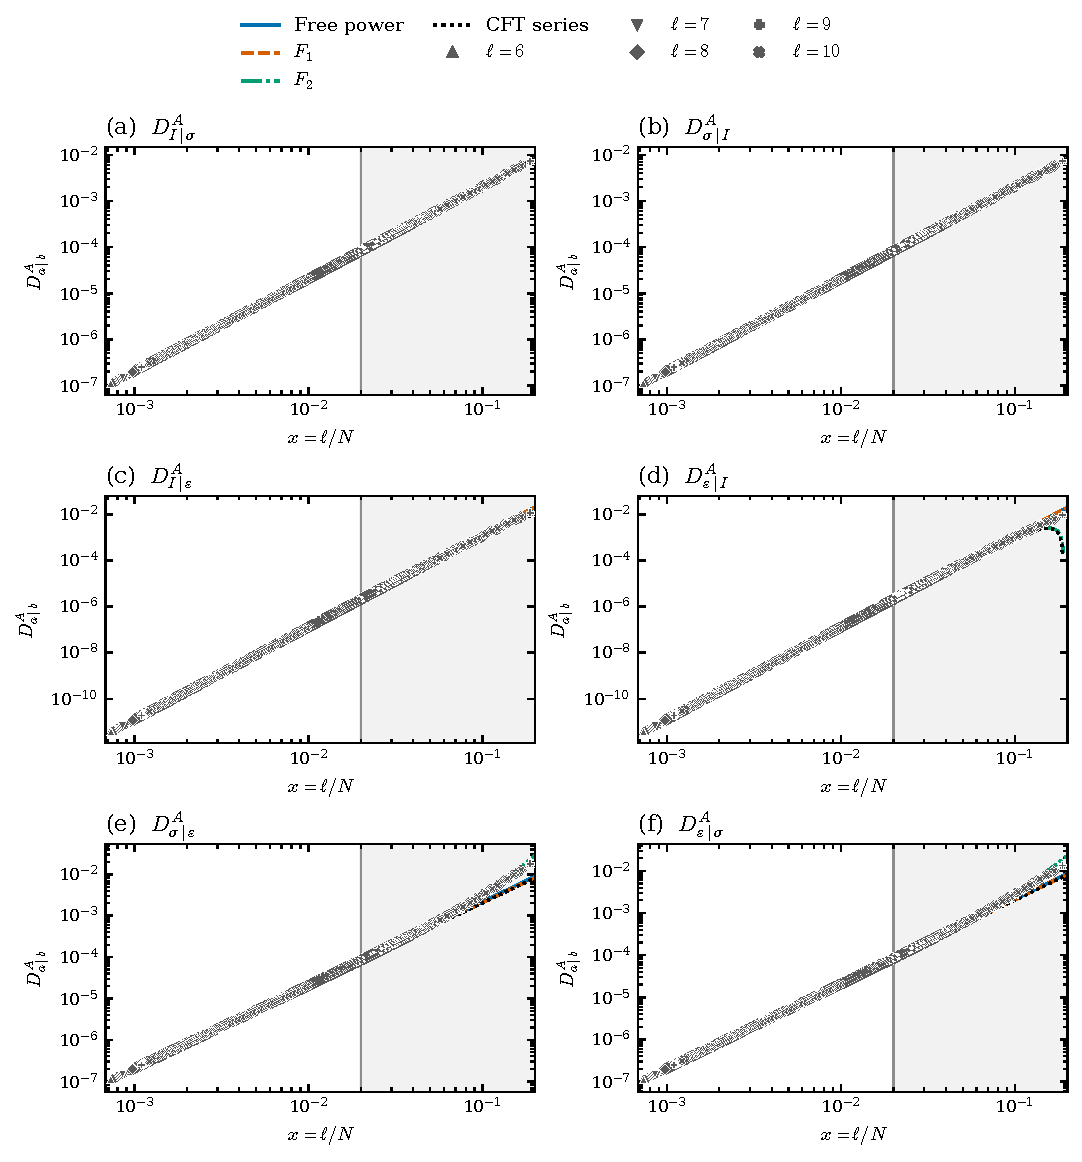
\includegraphics[width=.88\linewidth]{../figs/ising_small_value.pdf}
\caption{Both axes are logarithmic. Nonpositive values of an extrapolated truncated curve are omitted only from this logarithmic panel, while residual panels retain their predictions. Ising mixtures at $p=1/2$, $\ell=6,7,8,9,10$, and the chain-size set in Eq.~\eqref{eq:extended-grid}, with $32\leq N\leq8192$. There are 1645 displayed geometries per direction at $x\leq0.2$, of which 1255 satisfy $x\leq0.02$ and enter every fit. Marker shape identifies $\ell$; the vertical boundary and gray shading mark the fitting cutoff and excluded data. The periodic Ising Hamiltonian is $H=-\sum_jX_jX_{j+1}-\sum_jZ_j$; primaries use exact fermionic covariances, including the odd Ramond ground state for $\sigma$. Natural logarithms apply. Added sizes use the direct entropy remainder in Sec.~\ref{sec:stable-entropy}, with support cutoff $10^{-15}$. Blue solid is the free-power fit (two fitted parameters), orange dashed is $F_1$ (one), green dash--dot is $F_2$ (two), and black dotted is the supplied CFT series (zero). Powers and amplitudes use Eqs.~\eqref{eq:fit} and \eqref{eq:hierarchy}; all coefficients include powers of $\pi$. Fits minimize unweighted squared residuals in $D^A$. These curves use \texttt{scaling\_fit\_summary.csv}. The identical fits in Tables~\ref{tab:ising-small-parameters} and \ref{tab:ising-small-metrics} also have per-pair full-range and fitting-window views in Sec.~\ref{sec:pair-small_ising}.}
\label{fig:isingfits}
\end{figure}

\begin{figure}[p]\centering
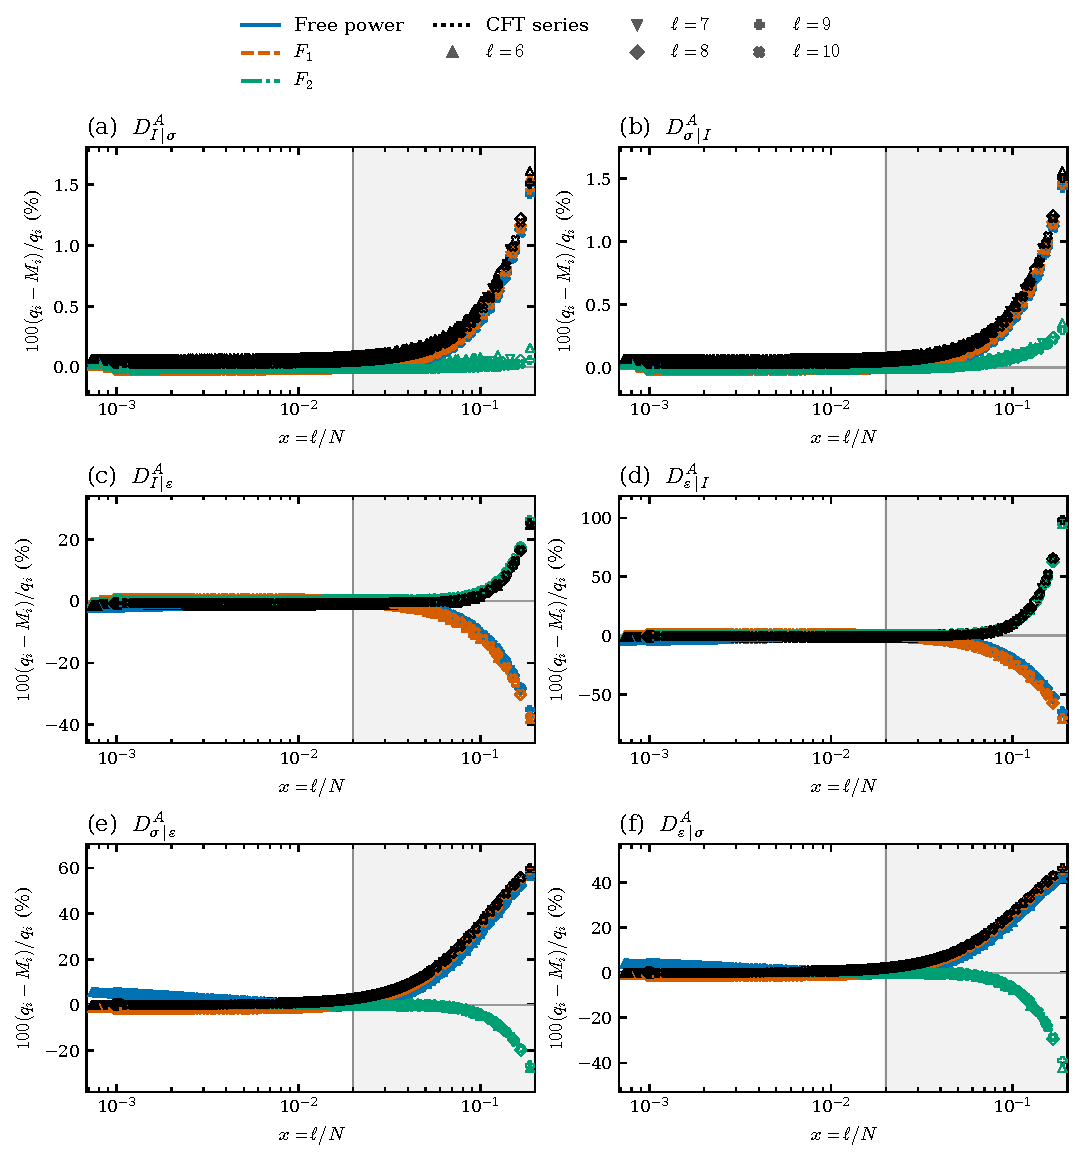
\includegraphics[width=.88\linewidth]{../figs/ising_small_residual.pdf}
\caption{The ordinate is $100(q_i-M_i)/q_i$ percent, with $q_i=D^A_i$ for a small interval and $q_i=\delta_i$ for a large interval; the horizontal zero line aids comparison. All four models have residual markers, colored as their curves. The residual ordinate is linear; the fraction axis is logarithmic. Ising mixtures at $p=1/2$, $\ell=6,7,8,9,10$, and the chain-size set in Eq.~\eqref{eq:extended-grid}, with $32\leq N\leq8192$. There are 1645 displayed geometries per direction at $x\leq0.2$, of which 1255 satisfy $x\leq0.02$ and enter every fit. Marker shape identifies $\ell$; the vertical boundary and gray shading mark the fitting cutoff and excluded data. The periodic Ising Hamiltonian is $H=-\sum_jX_jX_{j+1}-\sum_jZ_j$; primaries use exact fermionic covariances, including the odd Ramond ground state for $\sigma$. Natural logarithms apply. Added sizes use the direct entropy remainder in Sec.~\ref{sec:stable-entropy}, with support cutoff $10^{-15}$. Blue solid is the free-power fit (two fitted parameters), orange dashed is $F_1$ (one), green dash--dot is $F_2$ (two), and black dotted is the supplied CFT series (zero). Powers and amplitudes use Eqs.~\eqref{eq:fit} and \eqref{eq:hierarchy}; all coefficients include powers of $\pi$. Fits minimize unweighted squared residuals in $D^A$. These curves use \texttt{scaling\_fit\_summary.csv}. The identical fits in Tables~\ref{tab:ising-small-parameters} and \ref{tab:ising-small-metrics} also have per-pair full-range and fitting-window views in Sec.~\ref{sec:pair-small_ising}.}
\label{fig:isingresid}
\end{figure}

\begin{figure}[p]\centering
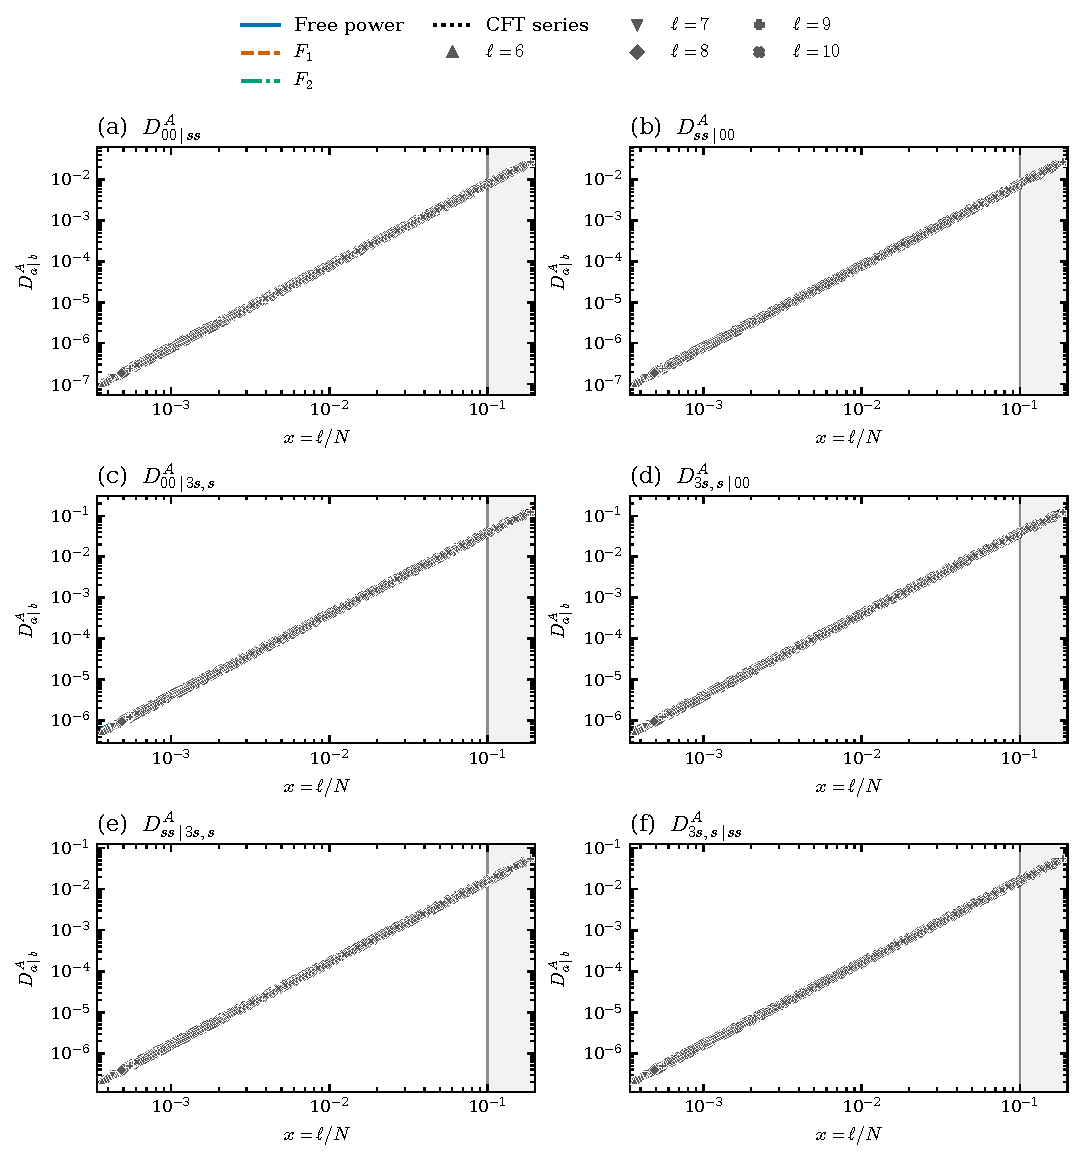
\includegraphics[width=.88\linewidth]{../figs/boson_small_value.pdf}
\caption{Both axes are logarithmic. Nonpositive values of an extrapolated truncated curve are omitted only from this logarithmic panel, while residual panels retain their predictions. Compact-boson mixtures at $p=1/2$, $\ell=6,7,8,9,10$, and the chain-size set in Eq.~\eqref{eq:extended-grid}, with $32\leq N\leq16384$. There are 625 displayed geometries per direction at $x\leq0.2$, of which 598 satisfy $x\leq0.1$ and enter every fit. Marker shape identifies $\ell$; the vertical boundary and gray shading mark the fitting cutoff and excluded data. The boson uses $s=1/\sqrt2$, $q=2$, charge codes $(0,0),(1,1),(3,1)$, $z_j=e^{2\pi i j/N}$, $w_1=0$, and $W=10^8$; moment algebra uses 100 digits through $N=256$ and 120 digits at the added sizes. Natural logarithms apply. Added sizes use the direct entropy remainder in Sec.~\ref{sec:stable-entropy}, with support cutoff $10^{-15}$. Blue solid is the free-power fit (two fitted parameters), orange dashed is $F_1$ (one), green dash--dot is $F_2$ (two), and black dotted is the supplied CFT series (zero). Powers and amplitudes use Eqs.~\eqref{eq:fit} and \eqref{eq:hierarchy}; all coefficients include powers of $\pi$. Fits minimize unweighted squared residuals in $D^A$. These curves use \texttt{scaling\_fit\_summary.csv}. The identical fits in Tables~\ref{tab:boson-small-parameters} and \ref{tab:boson-small-metrics} also have per-pair full-range and fitting-window views in Sec.~\ref{sec:pair-small_boson}.}
\label{fig:bosonfits}
\end{figure}

\begin{figure}[p]\centering
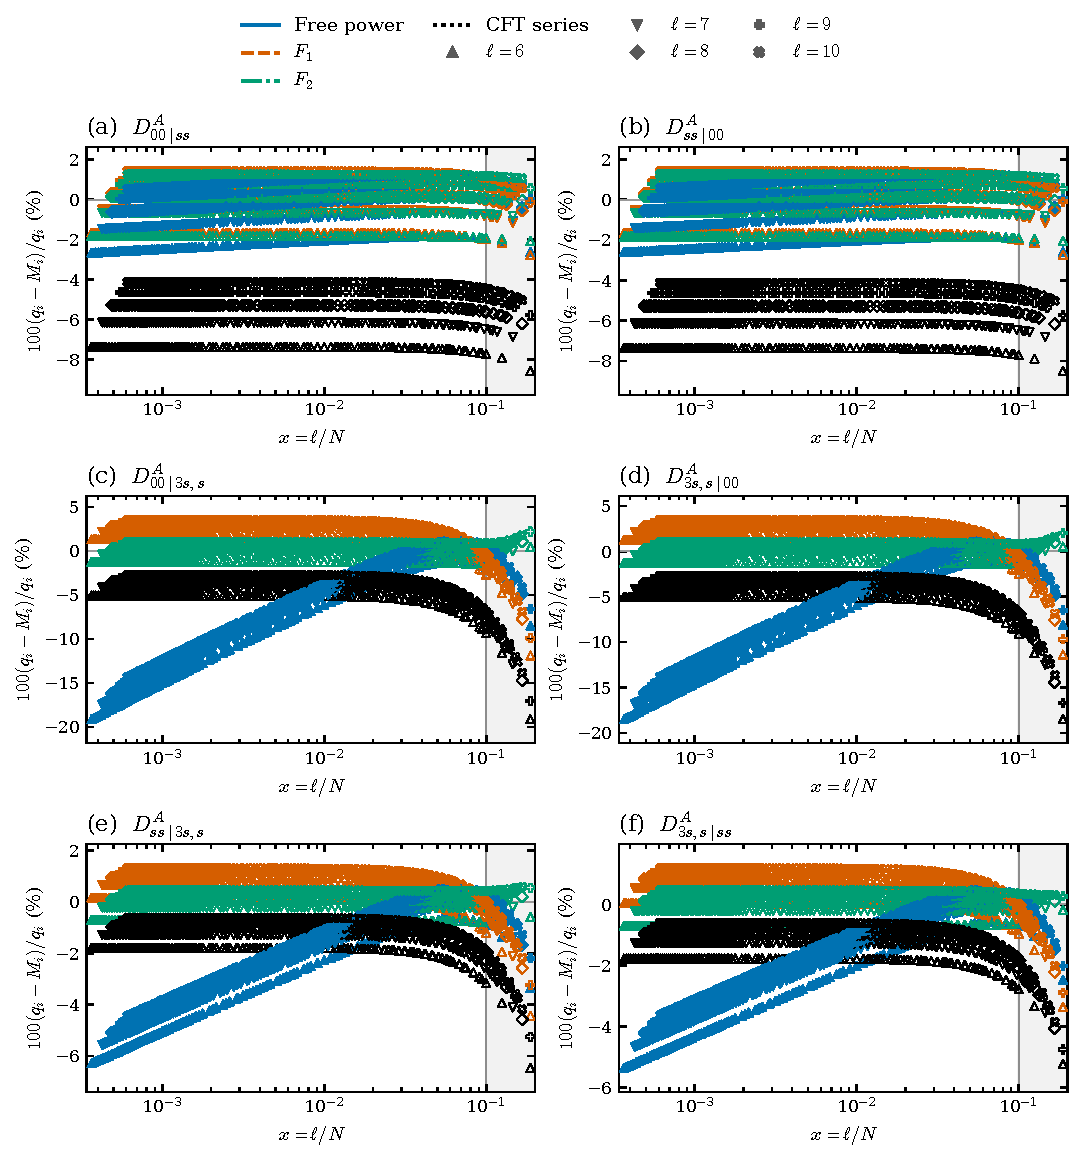
\includegraphics[width=.88\linewidth]{../figs/boson_small_residual.pdf}
\caption{The ordinate is $100(q_i-M_i)/q_i$ percent, with $q_i=D^A_i$ for a small interval and $q_i=\delta_i$ for a large interval; the horizontal zero line aids comparison. All four models have residual markers, colored as their curves. The residual ordinate is linear; the fraction axis is logarithmic. Compact-boson mixtures at $p=1/2$, $\ell=6,7,8,9,10$, and the chain-size set in Eq.~\eqref{eq:extended-grid}, with $32\leq N\leq16384$. There are 625 displayed geometries per direction at $x\leq0.2$, of which 598 satisfy $x\leq0.1$ and enter every fit. Marker shape identifies $\ell$; the vertical boundary and gray shading mark the fitting cutoff and excluded data. The boson uses $s=1/\sqrt2$, $q=2$, charge codes $(0,0),(1,1),(3,1)$, $z_j=e^{2\pi i j/N}$, $w_1=0$, and $W=10^8$; moment algebra uses 100 digits through $N=256$ and 120 digits at the added sizes. Natural logarithms apply. Added sizes use the direct entropy remainder in Sec.~\ref{sec:stable-entropy}, with support cutoff $10^{-15}$. Blue solid is the free-power fit (two fitted parameters), orange dashed is $F_1$ (one), green dash--dot is $F_2$ (two), and black dotted is the supplied CFT series (zero). Powers and amplitudes use Eqs.~\eqref{eq:fit} and \eqref{eq:hierarchy}; all coefficients include powers of $\pi$. Fits minimize unweighted squared residuals in $D^A$. These curves use \texttt{scaling\_fit\_summary.csv}. The identical fits in Tables~\ref{tab:boson-small-parameters} and \ref{tab:boson-small-metrics} also have per-pair full-range and fitting-window views in Sec.~\ref{sec:pair-small_boson}.}
\label{fig:bosonresid}
\end{figure}

